\documentclass{article}
\usepackage{amsmath, amssymb, mdwlist, graphicx, hyperref}
\usepackage{listings,color}
\usepackage{wrapfig}
\usepackage[usenames,dvipsnames]{xcolor}
\definecolor{gray}{rgb}{0.97,0.97,0.97}
\lstset{%
language=Python,%
%backgroundcolor=\color{gray},
emph={putpixel},
emphstyle=\bf,
tabsize=4,
framesep=5pt,
mathescape=true,
xleftmargin=2cm,
xrightmargin=2cm,
frame=lines,
%basicstyle=\ttfamily,
%keywordstyle=\color{Blue},
%commentstyle=\color{OliveGreen},
%stringstyle=\color{MidnightBlue},
columns=flexible,
%showstringspaces=false
}

\newcommand{\mpar}[1]{\marginpar{\textit{#1}}}
\newcommand{\norm}[1]{\Vert #1 \Vert}
\DeclareMathOperator{\argmax}{argmax}
\DeclareMathOperator{\argmin}{argmin}
\newenvironment{solution}{\paragraph{Solution.}$\,$ }{\vskip 3mm\hrule}
\newenvironment{exercise}[2]{\begin{verse}\textbf{Exercise #1 (#2pt).} }{
\end{verse}\medskip}
\newcommand{\bbR}{\mathbb{R}}
\newcommand{\bw}{\mathbf{w}}
\newcommand{\bx}{\mathbf{x}}
\newcommand{\bd}{\mathbf{d}}
\newcommand{\bb}{\mathbf{b}}
\newcommand{\by}{\mathbf{y}}
\newcommand{\bzero}{\mathbf{0}}
\newcommand{\bz}{\mathbf{z}}
\newcommand{\bSigma}{\mathbf{\Sigma}}
\newcommand{\bp}{\mathbf{p}}
\newcommand{\bm}{\mathbf{m}}
\newcommand{\bc}{\mathbf{c}}
\newcommand{\bM}{\mathbf{M}}
\newcommand{\bK}{\mathbf{K}}
\newcommand{\bD}{\mathbf{D}}
\newcommand{\bA}{\mathbf{A}}
\newcommand{\bX}{\mathbf{X}}
\newcommand{\bY}{\mathbf{Y}}
\newcommand{\bR}{\mathbf{R}}
\newcommand{\bI}{\mathbf{I}}
\newcommand{\bS}{\mathbf{S}}
\newcommand{\bT}{\mathbf{T}}
\newcommand{\balpha}{\boldsymbol{\alpha}}
\newcommand{\pt}[2]{\left(\begin{array}{c}#1\\#2\end{array}\right)}

\begin{document}
\title{MTAT.03.015 Computer Graphics (Fall 2013)\\
Exercise session III: Rasterization of Triangles}
\author{Konstantin Tretyakov, Ilya Kuzovkin}
\date{September 23, 2013}
\maketitle

Last week we've got a taste for how simple straight line segments can be drawn efficiently. Today we shall study the algorithm for rasterizing the simplest \emph{filled} shape -- the triangle. Due to its simplicity it is the most important primitive: models in 3D graphics are always decomposed into and rendered on a triangle-by-triangle basis. The speed with which each triangle is processed and rasterized is therefore key to the performance of a graphics card. Modern GPUs can handle around 2 \emph{billion} triangles per second\footnote{\url{http://goo.gl/fdGcR6}}.

The base code is provided in the \texttt{practice03.zip} archive on the course website\footnote{Alternatively, all lecture slides and practice session materials are also available on Github: \url{http://github.org/konstantint/ComputerGraphics2013}}. Download, unpack and open it. You will have to write all the code (except for the last bonus task) within the \texttt{triangles.cpp} file. Hence, you may submit your solution as just this single file (perhaps bundled into an archive with the bonus task solution).

\section{Basic Triangle Rasterization}


\begin{wrapfigure}{r}{0.4\textwidth}
\centering
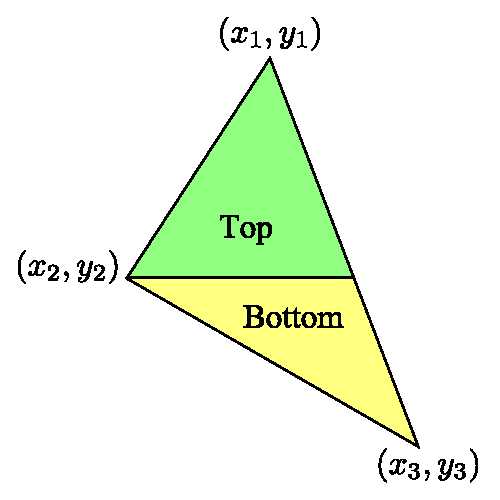
\includegraphics[width=0.35\textwidth]{triangle.pdf}
\end{wrapfigure}

Consider a triangle given by three points $\bp_1, \bp_2, \bp_3$. For simplicity in this exercise we shall assume that the coordinates of the vertices are integers\footnote{Note, though, that this simplification is not realistic: triangles rendered in most 3D applications would usually have non-integer vertex coordinates. You are welcome to think about how the algorithms discussed below should be adjusted to allow for sub-pixel accuracy.}.

Suppose the points are ordered from top to bottom. The triangle can then be split vertically into the ``top'' part (lines between $y_1$ and $y_2$) and the ``bottom'' part (lines $y_2+1$ to $y_3$).

To render each part, we will simply run along the edges using two simple line-rasterizers in parallel, filling all the pixels inbetween:

\begin{lstlisting}[escapechar=@]
   sort_points_vertically()
	@{\color{blue}// Step size along the X axis}@
	@{\color{blue}// for left and right edges}@
	$dx_\mathrm{A}$ = $(x_2 - x_1)/(y_2 - y_1)$
	$dx_\mathrm{B}$ = $(x_3 - x_1)/(y_3 - y_1)$
	$x_\mathrm{A}$ = $x_\mathrm{B}$ = $x_1$
	@{\color{blue}// Render the top part}@
	for $y$ in $[y_1\dots y_2]$:
		horizontal_line($x_\mathrm{A}$, $x_\mathrm{B}$, y)
		 $x_\mathrm{A}$ += $dx_\mathrm{A}$
		 $x_\mathrm{B}$ += $dx_\mathrm{B}$
	@{\color{blue}// Continue similarly for the bottom part}@
	@{\color{blue}// $\dots$}@
\end{lstlisting}

\begin{exercise}{1}{1}
Implement the above triangle rendering algorithm within the function \verb#simple_triangle#.

Hint: The point sorting routine and the \verb#horizontal_line# function are provided for your convenience.

Hint: The case where $y_1 = y_2$ must be taken care of specially.
\end{exercise}

\begin{exercise}{2*}{1}
You can make this algorithm purely integer-based using (a slightly modified) Bresenham's algorithm to track the edges. Devise a pure integer-based implementation for \texttt{simple} \verb#_triangle#. 

Hint: Note that in this case you may not make an assumption that the lines are ``non-steep'', hence you will need to represent the integral and the fractional parts of $dx$ in separate variables.
\end{exercise}

\section{Triangle Rasterization with Interpolation}
It is common to have \emph{attributes} associated with the vertices of the triangle. The simplest example is color. Suppose the first vertex has been assigned color red $(1,0,0)$, the second is green $(0,1,0)$ and the third one blue $(0,0,1)$. When rasterizing the triangle we would like to \emph{linearly interpolate} those values at every pixel. For example, the point lying exactly on the edge between the first and the second vertex should be dark yellow $(0.5, 0.5, 0)$, which is the color halfway between red and green. The point lying in the middle of the triangle should be gray $(0.33, 0.33, 0.33)$, an equal mixture of the three colors, etc.

We can modify the simple triangle algorithm to perform color interpolation as follows:
\begin{lstlisting}[escapechar=@]
	@{\color{blue}// ... }@
	@{\color{blue}// Step size for color for left and right edges}@
	$\mathbf{dc}_\mathrm{A}$ = $(\mathbf{c}_2 - \mathbf{c}_1)/(y_2 - y_1)$
	$\mathbf{dc}_\mathrm{B}$ = $(\mathbf{c}_3 - \mathbf{c}_1)/(y_2 - y_1)$
	$\mathbf{c}_\mathrm{A}$ = $\mathbf{c}_\mathrm{B}$ = $\mathbf{c}_1$
	@{\color{blue}// Render the top part}@
	for $y$ in $[y_1\dots y_2]$:
		gradient_line($x_\mathrm{A}$, $\bc_\mathrm{A}$, $x_\mathrm{B}$, $\bc_\mathrm{B}$, y)
		 $x_\mathrm{A}$ += $dx_\mathrm{A}$
		 $x_\mathrm{B}$ += $dx_\mathrm{B}$
		 $\bc_\mathrm{A}$ += $\mathbf{dc}_\mathrm{A}$
		 $\bc_\mathrm{B}$ += $\mathbf{dc}_\mathrm{B}$
	@{\color{blue}// Continue similarly for the bottom part}@
	@{\color{blue}// $\dots$}@
\end{lstlisting}

Here the values $\bc_1$, $\bc_2$, and $\bc_3$ are vectors representing the colors assigned to each vertex.

\begin{exercise}{3}{1}
Implement triangle rendering with color interpolation within the function \verb#color_triangle#.

Hint: The updated point sorting routine and the \verb#gradient_line# function are provided for your convenience.

Hint: Use the provided \verb#vector3f# class to represent colors.
\end{exercise}

\section{Textured Triangle}
Quite often, rather than (or in addition to) assigning colors to the vertices of a triangle, we shall assign \emph{texture coordinates} $(u_i, v_i)$. Texture coordinates indicate the location of a pixel within a \emph{texture image} that needs to be mapped to the given vertex of the triangle. When filling the triangle we shall interpolate texture coordinates in the same way as we did for colors.

That is, if in the previous algorithm we computed an interpolated color value $\bc = (r,g,b)$ for each pixel and set the pixel to that value:
\begin{lstlisting}[escapechar=@]
	al_put_pixel(x, y, $\bc$)
\end{lstlisting}
now we shall be computing an interpolated pair of texture coordinates $(u, v)$, and pick the corresponding pixel from the texture.
\begin{lstlisting}[escapechar=@]
	al_put_pixel(x, y, texture[(int)u, (int)v])
\end{lstlisting}


\begin{exercise}{4}{0.5}
Implement triangle rendering with texturing within the function \verb#textured_triangle#. For simplicity we shall use the same \texttt{vector3f} class here to represent texture coordinates (we simply ignore the third component of \texttt{vector3f}).

Hint: To modify \verb#color_triangle# into \verb#textured_triangle# you will only need to change the \verb#gradient_line# to, say, \verb#textured_line#.
\end{exercise}

\begin{exercise}{5*}{0.5}
When rendering a textured triangle, most pixels get associated with non-integer texture coordinates. In the previous exercise, however, you were simply rounding them to obtain the corresponding pixel from the texture. Because of that the resulting triangle looks somewhat ``jagged''. A much better way is to use \emph{bilinear interpolation} to blend the colors of four texture pixels surrounding the source texture location. Read about this technique and implement it in your \verb#textured_triangle# routine.
\end{exercise}

Figure below shows the screen you should observe after implementing the functions \verb#simple_triange#, \verb#color_triangle# and \verb#textured_triangle#.

\begin{figure}[h!]
\centering
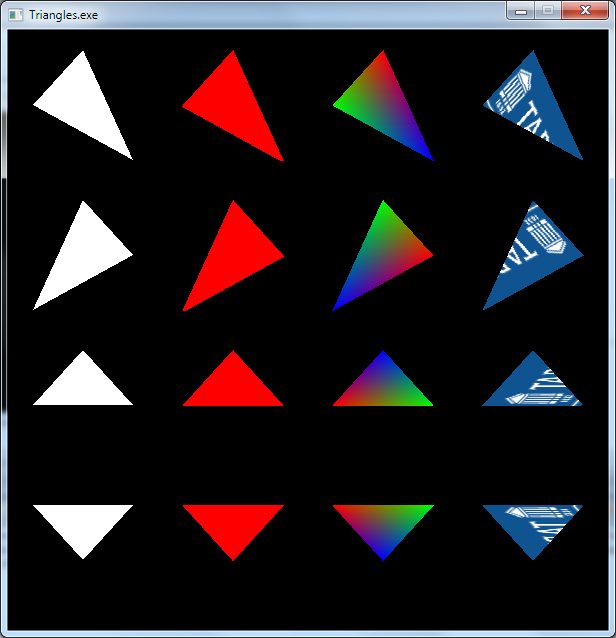
\includegraphics[width=0.85\textwidth]{screenshot.png}
%\caption{Result of exercises 1-5.}
\label{fig:screen}
\end{figure}

\section{Barycentric Coordinates}
You have seen the need to interpolate colors or texture coordinates along the triangle. In practice it is often necessary to interpolate \emph{both} color \emph{and} texture coordinates (perhaps for several textures), as well as a bunch of other things: normals, directions towards light sources, and custom variables.

The concept of \emph{barycentric coordinates} provides an easy way to wrap your head around all those interpolations. Recall from the lecture that every point $\bx$ inside the triangle $(\bp_1, \bp_2, \bp_3)$ can be represented as
$$
\bx = \lambda_1 \bp_1 + \lambda_2 \bp_2 + \lambda_3 \bp_3,
$$
with $\lambda_i \geq 0$, and $\lambda_1 + \lambda_2 + \lambda_3 = 1$. Importantly, such representation is unique.

That is, each point in the triangle has a unique tuple $(\lambda_1, \lambda_2, \lambda_3)$, corresponding to it, which is known as the \emph{barycentric coordinates} of that point with respect to the triangle. For example, the barycentric coordinates of $\bp_1$ are $(1, 0, 0)$. The barycentric coordinates of the point $\bp_2$ are $(0, 1, 0)$, and the coordinates of a point lying in the middle of an the edge between $\bp_1$ and $\bp_2$ are $(0.5, 0.5, 0)$.

Suppose now that some attributes (e.g. colors) $(\bx_1, \bx_2, \bx_3)$ are associated with the vertices of the triangle. It turns out now that for any pixel with barycentric coordinates $(\mu_1, \mu_2, \mu_3)$ within the triangle, the corresponding linearly interpolated color can be expressed simply as
$$
\mu_1 \bx_1 + \mu_2 \bx_2 + \mu_3 \bx_3.
$$
Consequently, it is only sufficient to interpolate the barycentric coordinates for each pixel. Interpolated value of any other attribute can be computed using those coordinates. In practice it is not an efficient method (it requires multiplications at each pixel), but it is a very clear way of reasoning about interpolated attributes.

\begin{exercise}{6}{0.5}
Consider the image below
\begin{center}
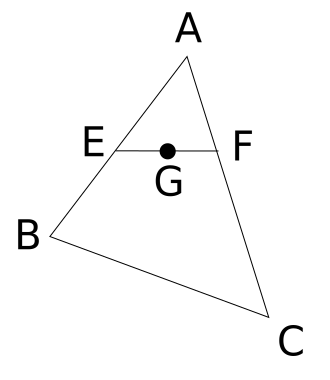
\includegraphics[width=0.3\textwidth]{barycentric}
\end{center}
Suppose $|AE| = |EB|$, $|FC| = 2|AF|$ and $|EG| = |FG|$. Compute the barycentric coordinates of the point $G$ with respect to the triangle $ABC$. Suppose that a real-valued attribute is associated with the vertices, such that $A$ is assigned value $10$, $B$ is assigned value $20$ and $C$ is assigned value $-10$. Use the barycentric coordinates you just found to compute the interpolated value of the attribute at point $G$.

Write the answers in the first lines of the \texttt{triangles.cpp} file as a comment.
\end{exercise}

\begin{exercise}{7*}{2}
In this bonus task we shall continue the topic of classical games. Another well known game is \emph{Breakout} (also known as Arkanoid, Bananoid, DX Ball\footnote{You can find both an on-line as well as the free Windows version of DXBall by following links from the Wikipedia page \url{http://en.wikipedia.org/wiki/DX-Ball}}, etc). Your task is to implement a simple version of Breakout:
\begin{itemize}
\item
The playing field initially consists of a $5\times 16$ wall of bricks, that can be broken using a ball. Player starts with 5 lives. Breaking each brick gives a point. When the ball touches the bottom of the screen the player loses a life. Game ends when either all bricks are broken or there are no more lives remaining.
\end{itemize}
This single level is sufficient for getting 2 points (although, of course, you are not limited in your creativity). 

Hint: Reuse the code you developed while implementing Pong.
\end{exercise}
\end{document}
